\documentclass[letterpaper]{tufte-handout}

\input{packages}
\usepackage[textsize=tiny,textwidth=1.2in]{todonotes}
\usepackage{xspace}
%\newcommand{\deaa}[1]{\todo{\textit{Daniel says:} #1}}
%\newcommand{\swlSide}[1]{\todo{\textit{Spencer says:} #1}}
\newcommand{\deaa}[1]{\xspace}
\newcommand{\swlSide}[1]{\xspace}

\newcommand{\swlSideNew}[1]{\todo{\textit{Spencer says:} #1}}



%\newcommand{\fg}[1]{\textcolor{green!50!black}{FG: {#1}}}
%\newcommand{\swl}[1]{\textcolor{red}{SL: {#1}}}
\newcommand{\swl}[1]{\xspace}
\newcommand{\da}[1]{\textcolor{purple}{DEAA: {#1}}}

\newtheorem{lemma}{Lemma}
\newtheorem{theorem}{Theorem}
\newtheorem{corollary}{Corollary}
\newtheorem{remark}{Remark}
\newtheorem{definition}{Definition}

\newcommand{\theMethod}{the Hermite timestepping method\xspace}
\newcommand{\Schrodinger}{Schr\"odinger\xspace}

\DeclareMathAlphabet{\mathpzc}{OT1}{pzc}{m}{it}

\DeclareMathOperator{\diag}{diag}


%\newcommand{\ctrlA}{{\mathfrak c}}
\newcommand{\ctrlA}{{\mathpzc c}}
\newcommand{\jfunc}{{\mathfrak j}}
\newcommand{\NTime}{{N_{\rm T}}}
\newcommand{\cost}{{\rm cost}}

\newcommand{\lagP}{\mathfrak{L}}

\newcommand{\Jcal}{\mathcal{J}}
\newcommand{\Lcal}{\mathcal{L}}
\newcommand{\Ocal}{\mathcal{O}}
\newcommand{\Fcal}{\mathcal{F}}

%
\newcommand{\ab}{{\mathbf a}}
\newcommand{\bb}{{\mathbf b}}
\newcommand{\db}{{\mathbf d}}
\newcommand{\eb}{{\mathbf e}}
\newcommand{\fb}{{\mathbf f}}
\newcommand{\gb}{{\mathbf g}}
\newcommand{\ib}{{\mathbf i}}
\newcommand{\jb}{{\mathbf j}}
\newcommand{\nb}{{\mathbf n}}
\newcommand{\pb}{{\mathbf p}}
\newcommand{\tb}{{\mathbf t}}
\newcommand{\rb}{{\mathbf r}}
\newcommand{\essb}{{\mathbf s}}
\newcommand{\yb}{{\mathbf y}}
\newcommand{\zb}{{\mathbf z}}
\newcommand{\qb}{{\mathbf q}}
\newcommand{\ub}{{\mathbf u}}
\newcommand{\vb}{{\mathbf v}}
\newcommand{\wb}{{\mathbf w}}

\newcommand{\Ab}{{\mathbf A}}
\newcommand{\Bb}{{\mathbf B}}
\newcommand{\Eb}{{\mathbf E}}
\newcommand{\Fb}{{\mathbf F}}
\newcommand{\Ib}{{\mathbf I}}
\newcommand{\Hb}{{\mathbf H}}
\newcommand{\Kb}{{\mathbf K}}
\newcommand{\Lb}{{\mathbf L}}
\newcommand{\Pb}{{\mathbf P}}
\newcommand{\Qb}{{\mathbf Q}}
\newcommand{\Rb}{{\mathbf R}}
\newcommand{\Ub}{{\mathbf U}}
\newcommand{\Tb}{{\mathbf T}}
\newcommand{\Xb}{{\mathbf X}}

\newcommand{\Abb}{\mathbb{A}}
\newcommand{\Bbbb}{\mathbb{B}}
\newcommand{\Ebb}{\mathbb{E}}
\newcommand{\Fbb}{\mathbb{F}}
\newcommand{\Ibb}{\mathbb{I}}
\newcommand{\Hbb}{\mathbb{H}}
\newcommand{\Kbb}{\mathbb{K}}
\newcommand{\Lbb}{\mathbb{L}}
\newcommand{\Nbb}{\mathbb{N}}
\newcommand{\Pbb}{\mathbb{P}}
\newcommand{\Qbb}{\mathbb{Q}}
\newcommand{\Rbb}{\mathbb{R}}
\newcommand{\Ubb}{\mathbb{U}}
\newcommand{\Tbb}{\mathbb{T}}
\newcommand{\Xbb}{\mathbb{X}}
\newcommand{\Ybb}{\mathbb{Y}}
\newcommand{\Zbb}{\mathbb{Z}}

\newcommand{\uh}{\hat{u}}
\newcommand{\vh}{\hat{v}}
\newcommand{\ph}{\hat{p}}
\newcommand{\qh}{\hat{q}}

\newcommand{\re}{{\rm Re}\,}
\newcommand{\im}{{\rm Im}\,}

\renewcommand{\arraystretch}{1.3}
%
\newcommand{\p}{\partial}
%
\newcommand{\eq}{\!\!\! = \!\!\!}
\newcommand{\om}{\omega}
%\newcommand{\divergence}{\nabla\cdot}
%\newcommand{\curl}{\nabla\times}

\newcommand{\lambdab}{\boldsymbol{\lambda}}
\newcommand{\psib}{\boldsymbol{\psi}}
\newcommand{\nub}{\boldsymbol{\nu}}
\newcommand{\mub}{\boldsymbol{\mu}}
\newcommand{\phib}{\boldsymbol{\phi}}
\newcommand{\Psib}{\boldsymbol{\Psi}}
\newcommand{\alphab}{\boldsymbol{\alpha}}
\newcommand{\thetab}{\boldsymbol{\theta}}

\newcommand{\rhob}{\boldsymbol{\rho}}
\newcommand{\kab}{\boldsymbol{\kappa}}
\newcommand{\etab}{\boldsymbol{\eta}}
\newcommand{\zetab}{\boldsymbol{\zeta}}
\newcommand{\sigmab}{\boldsymbol{\sigma}}
\newcommand{\omegab}{\boldsymbol{\omega}}

\newcommand{\zerob}{\boldsymbol{0}}
\newcommand{\epsilonb}{\boldsymbol{\epsilon}}

\newcommand{\deltab}{\boldsymbol{\delta}}
\newcommand{\Deltab}{\boldsymbol{\Delta}}

\newcommand{\forcing}{{\bf \mathcal{F}}}


\newcommand{\Gb}{{\mathbf G}}
\newcommand{\kb}{{\mathbf k}}
\newcommand{\sbold}{{\mathbf s}}
\newcommand{\ba}{\begin{array}}
\newcommand{\ea}{\end{array}}
\newcommand{\be}{\begin{equation}}
\newcommand{\ee}{\end{equation}}
\newcommand{\bd}{\begin{displaymath}}
\newcommand{\ed}{\end{displaymath}}
\newcommand{\pa}{\partial}
\newcommand{\f}{\frac}
\newcommand{\drp}{D^r_+}
\newcommand{\drm}{D^r_-}
\newcommand{\dqp}{D^q_+}
\newcommand{\dqm}{D^q_-}
\newcommand{\dtqn}{\widetilde{{D^q_0}} }
\newcommand{\dtrn}{\widetilde{{D^r_0}} }
\newcommand{\dqn}{D^q_0}
\newcommand{\drn}{D^r_0}
\newcommand{\erh}{E^r_{1/2}}
\newcommand{\eqh}{E^q_{1/2}}

\def\dpl{D_+}
\def\dmi{D_-}

\newcommand{\ubbar}{\bar{\mathbf{u}}}
\newcommand{\ubar}{\bar{u}}


% Grids
\newcommand{\xb}{\mathbf{x}}
\newcommand{\ybh}{\hat{\mathbf{x}}}
\newcommand{\xbh}{\hat{\mathbf{x}}}
\newcommand{\Ja}{J_{\alpha}}
\newcommand{\ga}{g_{\alpha}}
\newcommand{\Ma}{M_{\alpha}}

% Interpolation
\newcommand{\Nxy}{N_{\mathbf{x}\rightarrow\hat{\mathbf{x}}}}
\newcommand{\Nyx}{N_{\hat{\mathbf{x}}\rightarrow\mathbf{x}}}
\newcommand{\Nuv}{N_{\bar{\ub}_1\rightarrow\bar{\ub}_2}}
\newcommand{\Nvu}{N_{\bar{\ub}_2\rightarrow\bar{\ub}_1}}
\newcommand{\Nij}{N_{\bar{\ub}_i\rightarrow\bar{\ub}_j}}
\newcommand{\Nji}{N_{\bar{\ub}_j\rightarrow\bar{\ub}_i}}
\newcommand{\Px}{P}
\newcommand{\Pxh}{\hat{P}}

% Domains
\newcommand{\domp}{\Omega_{p}}
\newcommand{\domu}{\Omega_{\ub}}
\newcommand{\domv}{\Omega_{\vb}}
\newcommand{\domui}{\Omega_{\bar{\mathbf{u}}_i}}
\newcommand{\domuj}{\Omega_{\bar{\mathbf{u}}_j}}
\newcommand{\gamja}{\Gamma_{j0}}
\newcommand{\gamjb}{\Gamma_{j1}}
\newcommand{\gamia}{\Gamma_{i0}}
\newcommand{\gamib}{\Gamma_{i1}}

\newcommand{\C}{\mathbb{C}}
\newcommand{\R}{\mathbb{R}}


% Easier vectors and matrices
\newcommand*{\bmat}[1]{\begin{bmatrix} #1 \end{bmatrix}}
\newcommand*{\pmat}[1]{\begin{pmatrix} #1 \end{pmatrix}}


% Easier left and right parentheses and brackets
\newcommand{\lpar}{\left(}
\newcommand{\rpar}{\right)}
\newcommand{\lbra}{\left[}
\newcommand{\rbra}{\lright]}
\newcommand{\bracketed}[1]{\left[ #1 \right]}

% Unifying timestep notation
\newcommand{\stepDeriv}[3]{#1_{#2}^{(#3)}}

% For when something needs a citation but I don't have the reference yet
%\newcommand{\citeNeeded}[1][]{[Citation Needed]}
% Can add a note for if I have a citation in mind but don't have the bibtex entry yet
%\newcommand{\citeNeeded}{[Citation Needed]\xspace}
\newcommand{\citeNeeded}{ {\color{red} $\bigoasterisk$} }
%\newcommand{\thisCiteNeeded}[1]{[Citation Needed : #1]\xspace}
\newcommand{\thisCiteNeeded}[1]{{\color{red} $\bigoasterisk$}}

% Bra-Ket notation
\newcommand{\ket}[1]{|#1\rangle}
\newcommand{\bra}[1]{\langle#1|}
\newcommand{\braket}[2]{\langle#1|#2\rangle}

% Inner products
%\newcommand{\innerprod}[1]{\left\langle #1 \right\rangle}
\newcommand{\innerprod}[2]{\left\langle #1, #2 \right\rangle}
% Norms
\newcommand\norm[1]{\left\lVert#1\right\rVert}

\DeclareMathOperator{\Hess}{Hess}
\DeclareMathOperator{\tr}{Tr}
\DeclareMathOperator*{\minimize}{minimize}
\DeclareMathOperator{\CNOT}{CNOT}

% Easy derivatives (in the style of the physics package)
\newcommand{\dv}[3][]{\frac{d^{#1}#2}{d{#3}^{#1}}}
\newcommand{\pdv}[2]{\frac{\partial #1}{\partial #2}}
\newcommand{\inlinepdv}[2]{\partial #1 / \partial #2}


\newcommand{\nctrl}{{N_c}}
\newcommand{\nParPerCtrl}{{n_c}}
\newcommand{\target}{\textrm{Target}}

\title{A Short Introduction to Quantum Optimal Control}
\author[Spencer Lee]{IPAM NOT2025 Working Group 10, Spencer Lee}
\date{19 March 2025}  % if the \date{} command is left out, the current date will be used


\begin{document}

\maketitle% this prints the handout title, author, and date

\begin{abstract}
\noindent We first give a short definition of quantum states and operators, and explain how quantum states evolve in time. We then explain what quantum optimal control is and how to frame it as nonlinear programming (optimization) problem which can be solved computationally. Finally, we explain the GRAPE technique.
\end{abstract}



\section{Quantum Computing}
The state of a closed quantum system can be represented by a complex-valued state vector $\psib \in \C^N$. Each observable \sidenote{A quantity that can be physically measured.} of the system is associated with a Hermitian matrix $O \in \C^{N \times N}$. The eigenvalues of the operator are the possible outcomes of the measurement\sidenote{Because the matrix is Hermitian, the eigenvalues are real, which makes sense because the eigenvalues are physically measurable quantities.}, and the corresponding eigenvectors are the states for which that measurement will be observed. We may write the state vector in terms of the orthonormal eigenvectors of $O$:
\begin{equation}
    \psib = c_1 \psib_1 + c_2 \psib_2 + \dots + c_N \psib_N.
\end{equation}
Then $|c_i|^2$ gives the probability of observing the state $\psib_i$ when the system is measured, upon which the system is said to \emph{collapse} to the measured state. For this reason, the coefficients $\{c_i\}$ are called \emph{probability amplitudes}. Consequently, the length of the state vector is $\| \psib \|_2^2 = 1$ at all times because the probabilities of observing each possible outcome must sum to one. This also implies that the time evolution of the state vector is unitary, since unitary matrices preserve length.

In the quantum computing literature, states are often represented using bra ket notation, where we may denote a state by $\ket{\psi}$. 
the state $\psib \in \C^N$ represents $\ket{\psi}$ in a particular measurement basis. Similarly, a matrix $O$ represents the \emph{operator} $\hat{O}$ in a particular basis. In other words, $\ket{\psi}$ is just a way of labeling a physical state, whereas a corresponding state vector $\psib \in \C^N$ gives information on the outcomes of measuring the system. We switch between the two notations when convenient, but mostly stick to representing states as complex-valued vectors.\sidenote{$\ket{\psib}$ is called a \emph{ket}, and $\bra{\psib} \sim \psib^\dagger$ is called a \emph{bra}. Cutely, the \emph{bracket} $\braket{\psi_\alpha}{\psi_\beta} = \psib_\alpha^\dagger \psib_\beta$ represents an inner product. Many by-hand calculations can be simplified using inner products and orthonormality of eigenvectors, so this notation can be convenient when working with pen and paper.}

In this work, we only consider closed quantum systems. In a quantum computing context, this means considering only time scales short enough that there is no significant interaction between the quantum computer and the environment. Open quantum systems, which model the interaction between the quantum computer and the environment, are much larger and more computationally challenging, but the algorithms for performing quantum optimal control on them are essentially the same as for closed quantum systems.

\section{Governing Equation: \Schrodinger's Equation}

The time evolution of the state vector from an initial state $\psib_0$ in a closed quantum system is governed by \Schrodinger's equation\footnote{We always choose our units so that $\hbar=1$.}
\begin{equation} \label{eq:schrodinger}
    \frac{d}{dt}\psib(t) = -iH(t)\psib(t),\quad \psib(0) = \psib_0 \in \C^N,
\end{equation}
where $H(t) \in \C^{N \times N}$ is the Hamiltonian of the system, the matrix corresponding\sidenote{In the sense of observables, described in the previous section.} to the measurement of the total energy of a system.\sidenote{\Schrodinger's equation is a postulate of quantum mechanics. It cannot be derived, but the idea that the dynamics of a quantum system are determined by the linear operator corresponding to the energy of the system can be classically motivated; in Hamiltonian mechanics, the dynamics of a classical system are determined by the Hamiltonian function of the system, which usually gives the total energy of the system.}

In most quantum computing hardware, the Hamiltonian takes the form:
\begin{equation} \label{eq:hamiltonian_drift_control}
    H(t) = H_d + f_1(t)H_{c,1} + f_2(t)H_{c,2} + \dots + f_\nctrl(t)H_{c,\nctrl}.
\end{equation}
$H_d$ is called the \emph{drift Hamiltonian}, because even when the functions $f_1,\dots,f_\nctrl$ are all zero, the state vector still \emph{drifts} because of the dynamics caused by $H_d$.\sidenote{The term \emph{system Hamiltonian} is also used to describe $H_d$.} $H_{c,1},\dots,H_{c,\nctrl}$ are called the \emph{control Hamiltonians}, because in a quantum computer the \emph{control functions} $f_1,\dots,f_\nctrl$ correspond to the amplitude of laser pulses (or something similar) which we can program in order to \emph{control} the dynamics of the system.

\section{Defining the Quantum Optimal Control Problem}
Quantum optimal control refers to the process of manipulating the Hamiltonian in (\ref{eq:schrodinger}, \ref{eq:hamiltonian_drift_control}) to implement some desired behavior. The two most common types of quantum optimal control problems are state transfer problems and gate design problems.

\subsection{State Preparation Problems}
In a state preparation problem, we start from some known quantum state $\psib_0$ which can easily be prepared on a quantum computer\sidenote{Usually, the initial state is the ground state of the quantum computer, which the quantum computer naturally relaxes to over time}. We want to \emph{transfer} the state to some desired state $\psib_\target$ over some period of time $0 \leq t \leq T$. Because the Hamiltonian controls the dynamics of the system, do this by searching for a Hamiltonian which causes the desired dynamics.

In order to quantify the ``closeness'' of two quantum states, we use the \emph{fidelity} between the two states:
\begin{equation} \label{eq:fidelity}
    F(\psi_\alpha, \psi_\beta) = |\braket{\psi_\alpha}{\psi_\beta}|^2 = |\psib_\alpha^\dagger \psib_\beta|^2 = F(\psib_\alpha, \psib_\beta).
\end{equation}
The fidelity has several properties which make it a good way to quantify the ``closeness'' of two quantum states.
\begin{enumerate}
    \item The fidelity between two states $F(\psi_\alpha, \psi_\beta)$ is $1$ when $\psi_\alpha = \psi_\beta$, and $0$ when the two states are orthogonal.
    \item The fidelity does not depend on the \emph{global phase} of the states. That is, $F(e^{i\delta_\alpha}\psib_\alpha, e^{i\delta_\beta}\psib_\beta)$ for all $\delta_\alpha, \delta_\beta \in \R$. This is physically significant because the global phase of a state cannot be measured.\sidenote{This means that the states $\sqrt{2}^{-1}(\psib_0+\psib_1)$ and $e^{i\delta}\sqrt{2}^{-1}(\psib_0+\psib_1)$ are indistinguishable. However, we can measure a \emph{relative} phase, so the states $\sqrt{2}^{-1}(\psib_0+\psib_1)$ and $\sqrt{2}^{-1}(\psib_0+e^{i\delta}\psib_1)$ \emph{are} distinguishable, although their probability amplitudes have the same magnitude.}
\end{enumerate}
Then we can write our optimal control problem as
%\begin{fullwidth}
\begin{gather*}
    \minimize_{f_1,\dots,f_\nctrl}\ \  1 - |\psib_\target^\dagger, \psib(T)|^2, \\
    \textrm{where}\ \ \frac{d}{dt}\psib(t) = -i\left(H_d + \sum_{n=1}^\nctrl f_n(t)H_{c,n}\right)\psib(t),\quad \psib(0) = \psib_0 \in \C^N.
\end{gather*}
We are trying to find control functions $\{f_i\}$ which implement a Hamiltonian which minimizes the \emph{infidelity} between the initial state and the target state.

I have no idea how to solve this optimization problem computationally, since I have no idea how to program a computer to search over the spaces of arbitrary functions $f: \R \rightarrow \R$.\sidenote{If you know how to do this, please let me know!} And analytic solutions are only known for a select few problems that involve very small quantum systems. To solve the optimization problem computationally, we introduce the control vector $\thetab \in \R^{\nParPerCtrl\cdot\nctrl  }$ to parameterize the control functions. Each control function is a linear combination\sidenote{In principle, the dependence may be nonlinear, but using a linear dependence keeps the parameterization of the control functions simple. A linear dependence is also computationally useful because it makes taking the gradient of the control functions trivial.} of $\nParPerCtrl$ basis functions.\sidenote{In principle, the number of basis functions can be different for each control function, but keeping the number the same makes it easier to write.} For notational convenience, we can write the control vector in matrix form as $\Theta \in \R^{\nParPerCtrl \cdot \nctrl}$, with $\Theta_{j,k} = \thetab_{(j-1)\nParPerCtrl + k}$.
\begin{equation} \label{eq:control_pulse_ansatz}
    f_j(t;\thetab) = \sum_{k=1}^{\nParPerCtrl} \Theta_{j,k} b_{j,k}(t), \quad j = 1,\dots,\nctrl.
\end{equation}
The choice of the basis functions ${b_{j,k}}$ is called the \emph{control pulse ansatz}.

We can finally write our optimization problem as
\begin{gather}
    \minimize_{\thetab}\ \  1 - |\psib_\target^\dagger, \psib(T)|^2, \label{eq:optimization_problem}\\
    \textrm{where}\ \ \frac{d}{dt}\psib(t) = -i\left(H_d + \sum_{n=1}^\nctrl f_n(t;\thetab)H_{c,n}\right)\psib(t),\quad \psib(0) = \psib_0 \in \C^N. \nonumber
\end{gather}
\marginnote{The semicolon in $f(t;\thetab)$ just indicates that $\thetab$ does not change often like $t$ does. We optimize over $\thetab$, but we only ever solve \Schrodinger's equation for a constant value of $\thetab$.}
We are searching for control parameters $\thetab$ which determine the control functions $\{f_i(t;\thetab)\}$, which determine the Hamiltonian $H(t)$, which controls the dynamics of the system, in order to minimize the infidelity between $\psib(T)$ and the target state $\psib_\target$.

Written in terms of $\thetab$, the optimization problem is now a nonlinear programming (NLP) problem with no constraints, where \Schrodinger's equation is solved numerically to find $\psib(T)$ and evaluate the objective function in \eqref{eq:optimization_problem}. Constraints may be added, for example to keep the amplitude of the control functions below some maximum determined by experimental constraints. This NLP may be solved by direct-search methods\sidenote{E.g. Nelder-Mead.}, or by gradient-based methods.\sidenote{E.g., gradient descent, ADAM, or quasi-Newton methods such as L-BFGS.} True second-order Newton methods could also be used, but they require computing the Hessian of the objective function, which is very computationally expensive.


\subsection{Gate Design Problems}
Quantum gates are the basic building blocks of quantum algorithms. In this way, they are analogous to classical logic gates\sidenote{AND, OR, NOT, XOR, etc.}. Each gate is a unitary transformation which acts on a subsystem of the full quantum system.\sidenote{E.g., it operates on only a few qubits in a quantum computer consisting of many qubits.} An algorithm may be specified using a circuit diagram, which maps out the gates used in a quantum algorithm, which qubits they are applied to, and in what order.
\begin{figure*}
    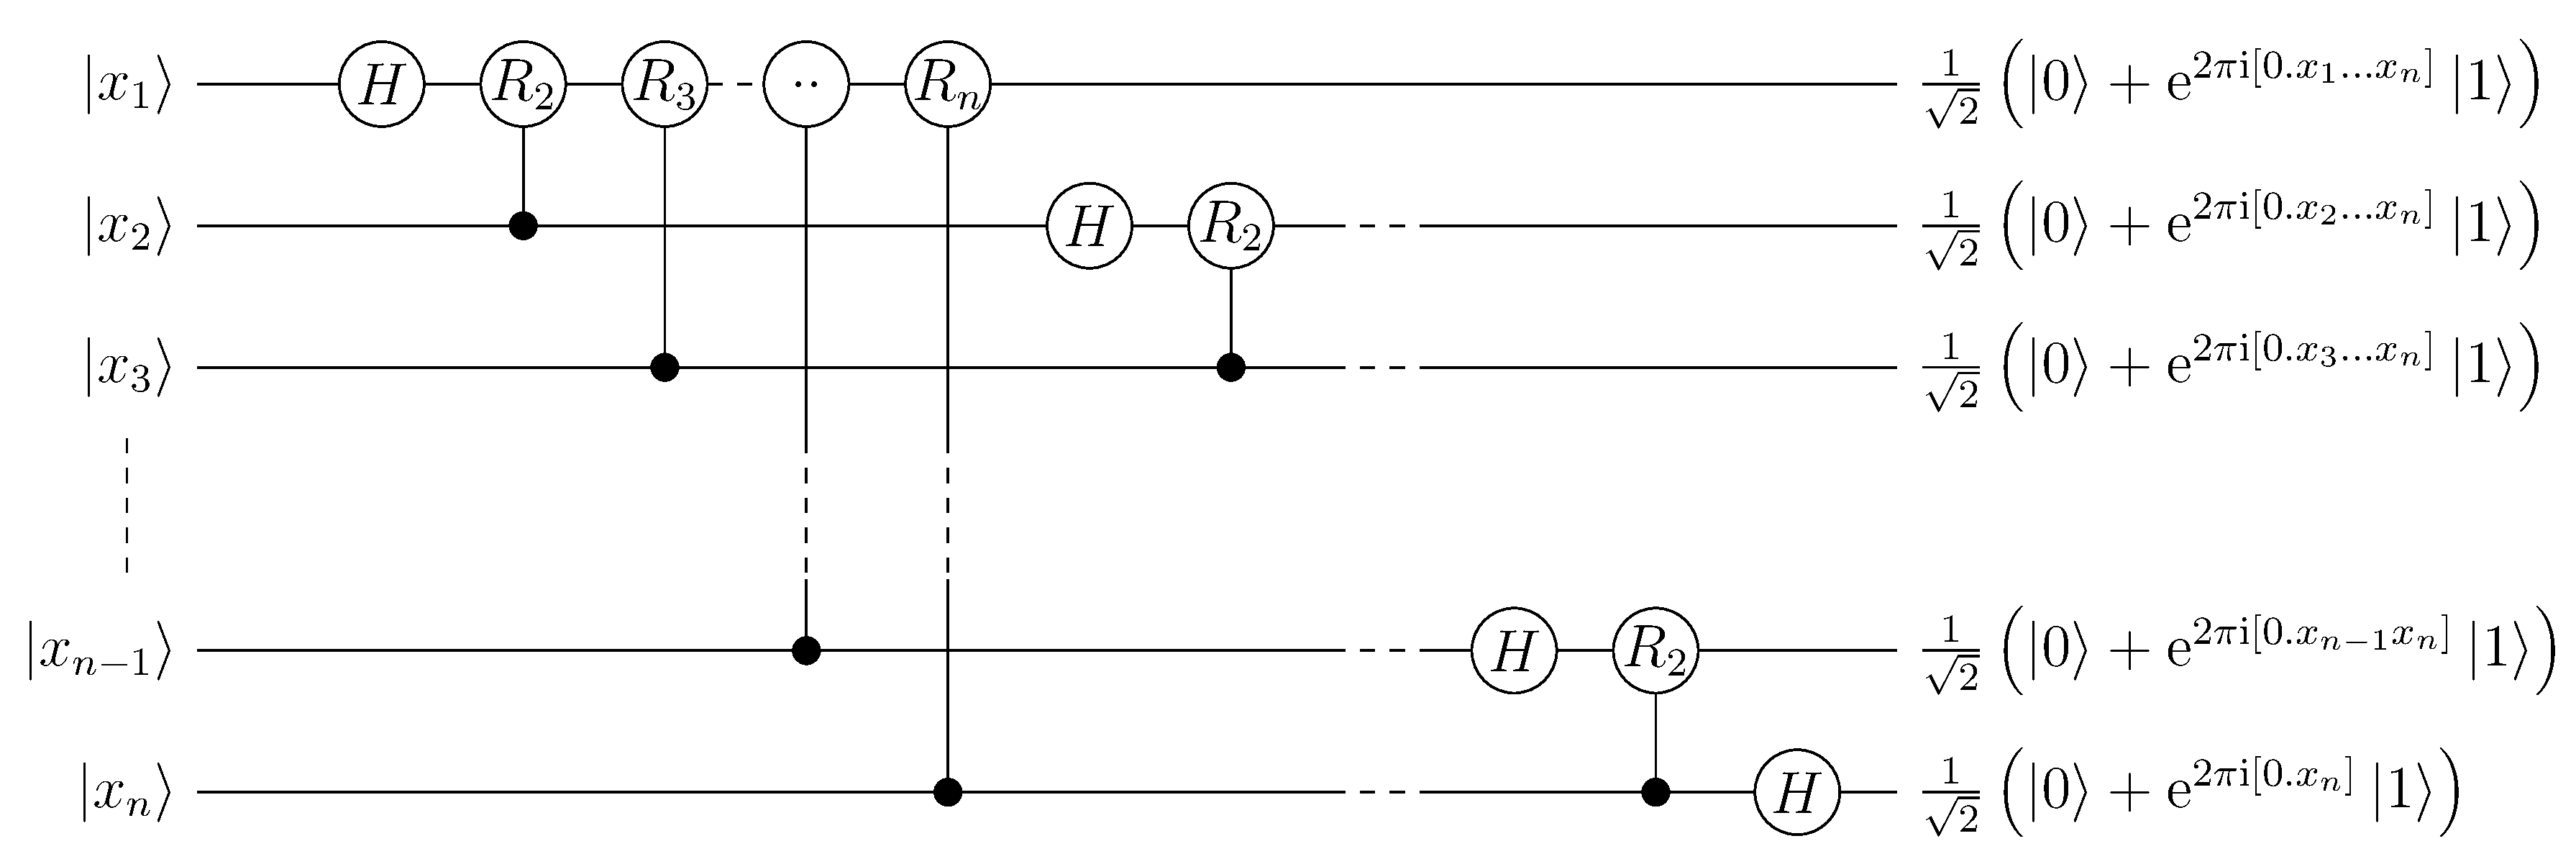
\includegraphics[width=0.9\linewidth, keepaspectratio]{QFT_circuit.png}
    \caption{Circuit diagram of the Quantum Fourier Transform algorithm.}
    \label{fig:qft_circuit}
\end{figure*}
To characterize a gate, it is sufficient to know how the gate transforms the elements of a basis of the subsystem. This allows us to specify a gate using a truth table, the same way we would specify a classical logic gate. For example, the truth table of a CNOT (Controlled NOT) gate is given in table \ref{tab:cnot}, and the matrix representation of the gate (i.e. the unitary transformation it applies, in the standard/computational basis) is
\begin{margintable}
\centering
\begin{tabular}{cc}
\toprule 
Initial State & Final State \\
\hline
$\ket{00}$ & $\ket{00}$ \\
$\ket{01}$ & $\ket{01}$ \\
$\ket{10}$ & $\ket{11}$ \\
$\ket{11}$ & $\ket{10}$ \\
\bottomrule 
\end{tabular}
\caption{Truth table that defines a CNOT gate.}
\label{tab:cnot}
\end{margintable}
\renewcommand{\arraystretch}{0.85} % Adjust vertical spacing of matrix
\begin{equation*}
    \CNOT\psib =  \begin{bmatrix}
        1 & 0 & 0 & 0  \\
        0 & 1 & 0 & 0  \\
        0 & 0 & 0 & 1  \\
        0 & 0 & 1 & 0  \\
    \end{bmatrix}
    \psib.
\end{equation*}

Roughly speaking, this is very similar to the state preparation problem, only now we are looking for a Hamiltonian which transfers several initial states to several corresponding target states. Strictly speaking, we are looking a Hamiltonian which generates a target unitary matrix $U_\target$. To see why optimizing for  a specific target unitary matrix is different than optimizing the ability of the unitary to prepare several final states from several initial states, consider the unitaries $U_A = \left[\begin{smallmatrix} 0 & 1 \\ 1 & 0 \end{smallmatrix}\right]$ and $U_B = \left[\begin{smallmatrix} 0 & 1 \\ i & 0 \end{smallmatrix}\right]$. We have $U_A \ket{0} = \ket{1}$, $U_A\ket{1}=\ket{0}$, $U_B\ket{0}=i\ket{1}$, $U_B\ket{1}=\ket{0}$. Because the global phase of a state cannot be measured, from a multiple state preparation point of view, the two unitaries both ``perfectly'' perform the state preparations $\ket{0} \rightarrow \ket{1}$, $\ket{1} \rightarrow \ket{0}$. The unitaries create different relative phases (which are measurable) when they operate on states other than the initial states in the state preparation problems: $U_A\sqrt{2}^{-1}\left(\ket{0}+\ket{1}\right)=\sqrt{2}^{-1}\left(\ket{1}+\ket{0}\right)$, $U_B\sqrt{2}^{-1}\left(\ket{0}+\ket{1}\right)=\sqrt{2}^{-1}\left(i\ket{1}+\ket{0}\right).$

When we say a Hamiltonian generates a unitary matrix, we mean it in the the dynamics caused by the Hamiltonian (according to \Schrodinger's equation) can by represented by a unitary time-evolution matrix $U(t)$:
\begin{equation*}
    \psib(t) = U(t)\psib_0 = e^{-i\int H(t)dt}\psib_0.
\end{equation*}
We want to choose a Hamiltonian (parameterized through $\thetab$), which over a period of time $0 \leq t \leq T$ generates a unitary $U(T)$ that is ``close'' to $U_\target \in \C^{N \times N}$. As before, we need a way to quantify the ``closeness`` of two unitaries. We use the \emph{gate infidelity}: 
\begin{equation}
F(U_\alpha, U_\beta) = \frac{1}{N^2}|\langle U_\alpha,U_\beta\rangle_F|^2 = \frac{1}{N^2}|\tr[U_\alpha^\dagger U_\beta]|^2.
\end{equation}
\marginnote{The Frobenius inner product $\langle A, B \rangle_F = \tr[A^\dagger B]$ can be computed simply as $\sum_{j,k} \overline{A}_{j,k}B_{j,k}$.}
As with the state fidelity, the gate infidelity takes a value between $0$ and $1$, is invariant to changes in the global phase of the unitaries.

Just as we did with state preparation problems, we parameterize the control functions in terms of a control vector $\thetab$ so we can formulate the quantum optimal problem as an NLP problem, which can be solved computationally.
\marginnote{$I_N$ denotes the $N$ by $N$ identity matrix.}
\begin{gather}
    \minimize_{\thetab}\ \  1 - \frac{1}{N^2}|\tr[U_\target^\dagger, U(T)]|^2, \label{eq:gate_optimization_problem}\\
    \textrm{where}\ \ \frac{d}{dt}U(t) = -i\left(H_d + \sum_{n=1}^\nctrl f_n(t;\thetab)H_{c,n}\right)\psib(t),\quad U(0) = I_{N}. \nonumber
\end{gather}
\section{GRAPE Optimization}
Optimizing even a two-qubit state transfer or gate design problem is moderately challenging, and three-qubit problems are quite difficult. \sidenote{Especially when the qubits are not treated as true two-level systems, but as 3 or 4 level systems, which is more accurate (technically, for most quantum computing architectures each qubit has an infinite number of levels).} As the systems become more difficult to control, more control parameters are typically needed in order to find a suitable set of control functions. The increased number of control parameters make the optimization more challenging do to the increased number of search dimensions, but gradient-based methods excel at navigating high-dimensional optimization landscapes.\sidenote{Although as the number of qubits increases, many optimization tasks suffer from the \emph{barren plateau} problem, which makes optimization extremely difficult even with gradient-based methods.} To use these methods, we need to be able to compute the gradient. A naive way is to approximate the partial derivatives of the objective function using finite differences, e.g.
\begin{equation*}
    \pdv{\Jcal}{\theta_n} \approx \frac{\Jcal(\thetab + h \boldsymbol{e}_n) - \Jcal(\thetab)}{h},
\end{equation*}
\marginnote[-0.4in]{We denote the $n$-th vector in the standard basis by $\boldsymbol{e}_n$.}
but then the gradient is inexact, and most importantly, computing the gradient a single time requires solving at least as many \Schrodinger equations as there are control parameters.

The GRAPE (\textbf{GR}adient \textbf{A}scent \textbf{P}ulse \textbf{E}ngineering) method\cite[-0.6in]{khaneja_2005} cleverly computes the gradient exactly, and with a cost of solving only two \Schrodinger equations, regardless of the number of control parameters. It does this by using a piecewise constant control pulse ansatz, where gate duration is divided into $\nParPerCtrl$ time intervals of width $\Delta t = T/\nParPerCtrl$, and the control functions are constant during that time interval. Specifically, in \eqref{eq:control_pulse_ansatz}, the basis functions are
\[
    b_{j,k}(t) = \begin{cases}
     1, & \text{if }\ (k-1)\frac{T}{\nParPerCtrl} \leq t  < k\frac{T}{\nParPerCtrl} \\
     0, & \text{otherwise}
    \end{cases}
\]
\begin{marginfigure}
    \begin{tikzpicture}
    \begin{axis}[
        width=2.6in,
        height=2in,
        axis x line=middle,
        axis y line=middle,
        xlabel={$t$}, ylabel={$f_1(t;\thetab)$},
        xtick={1,2,3,4,5,6,7},
        xticklabels={},
        ytick=\empty,
        ymin=-1, ymax=1, xmin=0, xmax=7,
        samples=100,
        enlargelimits=true,
        xlabel style={at={(axis cs:8.25,0)}, anchor=east}, % Move x label to the right
        ylabel style={at={(axis cs:0,1.2)}, anchor=south}, % Move y label above
        clip=false,
        axis equal=false,
    ]
        \addplot[
            thick,
            const plot mark left,
            domain=0:3,
            range=-1:1,
        ]
        coordinates {
            (0,1) (1,0.7) (2,-0.2) (3,0.-0.4) (4,-1) (5,-0.3) (6, 0.4) (7,0)
        };
        
        % Width annotation
        \draw[|<->|, thick] (axis cs:6,0.45) -- (axis cs:7,0.45);
        \node[anchor=south] at (axis cs:6.5,0.45) {$\Delta t$};

        % Height annotation
        \draw[|<->|, thick] (axis cs:2.2,0.7) -- (axis cs:2.2,0);
        \node[anchor=west] at (axis cs:2.2,0.35) {$\theta_2$};
    \end{axis}
\end{tikzpicture}
    \caption{An example of a piecewise constant control function, the kind which the GRAPE method uses.}
\end{marginfigure}
Simply stated, $\Theta_{j,k}$ is the amplitude of the $j$-th control function during the $k$-th time interval.\sidenote[][0.25in]{This control pulse ansatz may seem arbitrary, but the control functions are usually shaped using arbitrary waveform generators, for which the idealized output \emph{is} piecewise constant.}

For simplicity, we will consider a problem with only one control Hamiltonian, and no drift Hamiltonian.
\[
    \frac{d}{dt}U(t) = -if_1(t;\thetab)H_{c,1} U(t),\quad U_0 = I_{N}.
\]
Because the Hamiltonian is constant across each time interval, the time evolution across each interval can be computed using matrix exponentials. And we can write the time evolution across the whole duration as
\begin{equation} \label{eq:grape_unitaries}
    U(T) = U_\nParPerCtrl \cdots U_1 U(0) = e^{-i\theta_\nParPerCtrl H_{c,1} T / \nParPerCtrl} \cdots e^{-i\theta_1 H_{c,1} T / \nParPerCtrl} U(0).
\end{equation}
Now, the partial derivatives of the gate infidelity are
\begin{fullwidth}
\begin{equation} \label{eq:infidelity_pdv}
    \hspace*{-1in} \pdv{}{\theta_n}\left(1 - \frac{1}{N^2}\left|\tr\left[U_\target^\dagger U(T)\right]\right|^2\right) = -\frac{2}{N^2}\re\left(\tr\left[U_\target^\dagger \pdv{U(T)}{\theta_n}\right] \tr\left[U_\target^\dagger U(T)\right]\right).
\end{equation}
\end{fullwidth}
Performing the matrix multiplications and evaluating the traces in the above expression is cheap, but computing $\partial U(T) / \partial \theta_n$\sidenote[]{$\partial U(T) / \partial \theta_n$ is sometimes called a \emph{sensitivity.}} for each $n=1,\dots,\nParPerCtrl$ is expensive. Naively, they be obtained for each $\theta_n$ by solving a system of ODEs\sidenote{Perhaps we could have suspected this intuitively. Changing a control parameter changes the dynamics, so to know how the state at the end of the dynamics changes with respect to each control parameter we need to look at a new dynamical system for each control parameter.} similar to \Schrodinger's equation, but with a forcing term:\sidenote{This is actually done in the GOAT (\textbf{G}radient \textbf{O}ptimization) of \textbf{A}nalaytic Con\textbf{T}rols method.\cite{Machnes_2018}}
\[
    \frac{d}{dt}\pdv{U(t)}{\theta_n} = -if_1(t;\thetab)H_{c,1}\pdv{U(t)}{\theta_n} -i\pdv{f_1(t;\thetab)}{\theta_n}H_{c,1}U(t).
\]
But, because only the $n$-th unitary in \eqref{eq:grape_unitaries} depends on $\theta_n$, we can write $\partial U(T)/\partial \theta_n$ analytically as the simple expression
\[
\pdv{U(T)}{\theta_n} = -i\Delta tU_\nParPerCtrl \cdots U_{n+1}H_{c,1}U_n U_{n-1} \cdots U_1 U(0)
\]
Evaluating the partial derivative only involves inserting one extra matrix multiplication into the sequence of unitaries that we apply to $U(0)$ in order to get $U(T)$. Even better, we can write
\[
    U_\target^\dagger U(T) = \left(U_{n+1}^\dagger \cdots U_\nParPerCtrl^\dagger U_\target\right)^\dagger \left( U_n \cdots U_1 U(0)\right),
\]
and
\begin{fullwidth}
\begin{equation} \label{eq:grape_fold}
    \hspace{-2in}
    U_\target^\dagger \pdv{U(T)}{\theta_n} = -i\Delta t \left(U_{n+1}^\dagger \cdots U_\nParPerCtrl^\dagger U_\target\right)^\dagger H_{c,1}\left( U_n \cdots U_1 U(0)\right). 
\end{equation}
\end{fullwidth}
Then the procedure is to first compute $U(T) = U_\nParPerCtrl \cdots U_1 U(0)$.
Then, for $n = \nParPerCtrl,\dots,1$, use \eqref{eq:grape_fold} to compute $U_\target^\dagger (\inlinepdv{U(T)}{\theta_n})$. Because $U_{n+2}^\dagger\cdots U_\nParPerCtrl^\dagger U_\target$ and $U_{n-1}\cdots U_1 U(0)$ were already computer during the previous iteration, this only requires computing two matrix exponentials\sidenote{The matrix exponentials $U_1,\dots,U_n$ may computed once and stored, if there is sufficient memory available.} and performing three matrix-matrix multiplications, which is much less expensive than computing $\nParPerCtrl$ matrix exponentials\sidenote{Computing matrix exponentials is a computationally expensive operation, which is a drawback of the GRAPE method.} and performing $\nParPerCtrl+1$ matrix-matrix multiplications, which is cost of computing and multiplying all the unitaries in \eqref{eq:grape_fold}. During each iteration, once we have computed $U_\target^\dagger \inlinepdv{U(T)}{\theta_n}$ we can use \eqref{eq:infidelity_pdv} to compute the $n$-th partial derivative of the objective function (the infidelity). This concludes the method.

The GRAPE method was an important development, made around 2005. Since then, major improvements have been made, but modern developments in \emph{open-loop}\sidenote{In quantum optimal control, open-loop means completely simulation-based, with no experimental feedback. If there is experimental feedback, the method is called a closed-loop method.} quantum optimal control generally still rest on doing some kind of forward evolution, adjoint evolution scheme which produces exact gradients and does not scale heavily in cost with the number of control parameters.

The GRAFS (\textbf{GR}adient \textbf{A}scent in \textbf{F}unction \textbf{S}pace) method\cite{Lucarelli_2018} uses a similar technique as the GRAPE method; the control functions are piecewise constant, and the time evolution is performed using matrix exponentiation, which allows the gradient to be computed analytically and cheaply (using a forward solve and an adjoint solve). The major difference is that although the control pulses are piecewise constant, the control parameters do not correspond directly to the amplitudes of the control functions across each time interval. Instead, the control functions are parameterized in terms of continuous basis functions, as we did in \eqref{eq:control_pulse_ansatz}. The control functions are then discretized into piecewise constant functions, and the relationship between the control parameters and the discretized function amplitudes is used used to compute the gradient in an efficient way, similar to the GRAPE method.
\section{Disclaimers}
These notes were made quickly, without much proofreading. Please let me know if you find any mistakes!

I made many simplifications to make this handout more accessible. For example, qubits are two-level systems, but real hardware implementations of qubits are often infinite-level systems. We deal with this by including a couple of the lowest energy levels in our model, and adding to our objective function a term that penalizes the population of the excited states beyond the first two energy levels.


\section{Questions}
I have some questions I can't answer because I don't know enough about classical optimal control theory. I would appreciate any input from people more familiar with classical optimal control!
\begin{enumerate}
    \item What would the Hamilton-Jacobi-Bellman equations look like for a quantum optimal control problem, and why don't we solve the quantum optimal control problem by solving the Hamilton–Jacobi–Bellman equations?\sidenote{My guess is that it has to do with the curse of dimensionality.}
    \item Are the GRAPE method and similar methods (methods that use a forward/adjoint scheme to compute the gradient) the same as Pontryagin's maximum principle? If not, why don't we use it?\sidenote{According to section 3 of the GRAFS paper,\cite{Lucarelli_2018} GRAPE is essentially Pontryagin's maximum principle with trivial costate dynamics.}
\end{enumerate}


\bibliography{bibliography}
\bibliographystyle{plainnat}


\end{document}